%to compile, run "latex foo.tex"
%then you can view the dvi file with "xdvi foo.div" or yap on windows (?)
%or convert to pdf with "dvipdf foo.div" or "dvips -Pcmz foo.dvi -0 foo.ps" to postscript
%Or, just run "pdflatex foo.tex"

\documentclass{article}
\usepackage[pdftex]{graphicx}
\DeclareGraphicsExtensions{.pdf, .png, .jpg}
\graphicspath { {images/} }
\begin{document}


\subsection{Introduction}
Small is beautiful\cite{albaker2009survey} . 

%for a two column figure
\begin{figure*}
	\caption{a picture.}
	\label{fig:09Rahim}
	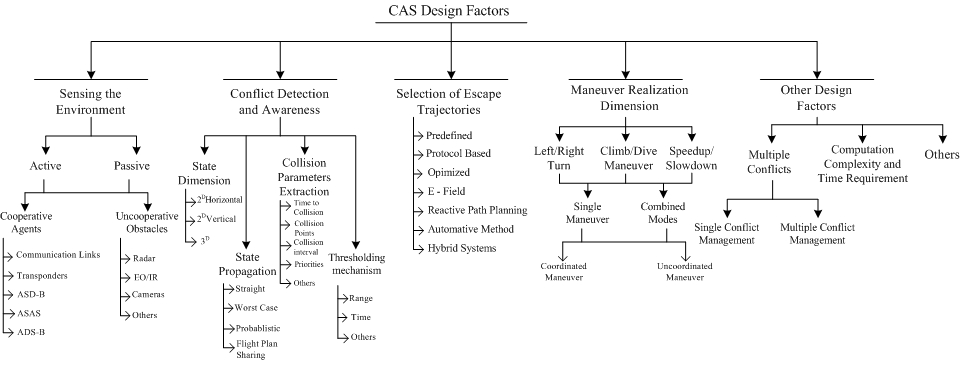
\includegraphics [width=1\textwidth] {09RahimCasDesign}
\end{figure*}

%for a image to fit in one column
%caption at bottom
%note, label must be below caption
\begin{figure}
	\includegraphics [width=1\columnwidth] {nameofpicture}
	\caption{a picture}
	\label{fig:something}
\end{figure}

\bibliographystyle{plain}
\bibliography{mybib}

%Bibliography time!!
%\begin{thebibliography}{99}

%\bibitem{unique}
%	Author,
%	\emph{some title}.
%	Publisher, State, edition blah blah.	

%\end{thebibliography}


\end{document}
